\section{Results}
\label{sec:results}
\subsection{Performance metrics}

In the following, we present results for the video retrieval and triplet 
metrics.
We report results on both the dialog and narration data.
In the case of the narration data the scores are not confounded by
speaker-based clues, which is an indication that the model possibly
learned to detect some aspects of utterance meaning. 

\paragraph{Pre-training and fine-tuning}
Results on different pre-training configurations are presented in Figure 
\Cref{fig:pretraining}.
The best overall performance on both the dialog and the narration data is 
achieved with a model where both the video and audio encoder are pre-trained 
before being fine-tuned on our data.

A pre-trained video encoder leads to higher gains on the dialog validation 
data, whereas for model generalization on the narration data we observe that a 
pre-trained audio encoder is more important. 

A model that is trained on scratch using only our data performs still 
substantially above chance on all metrics ($0.1$ for recall@10 and $0.5$ for 
triplet accuracy). \todo{MN: Do we maybe want to add the chance (random 
guessing) baselines into the plots?}

To further understand and disentangle the effects of audio pre-training and 
fine-tuning, we train a model with frozen parameters of the 
\textsc{wav2vec} 
module (\Cref{fig:freeze_wav2vec}). We find that if we don't allow a 
fine-tuning of the \textsc{wav2vec} module, performance decreases substantially 
on all 
metrics. In other words, best performance is only achieved with pre-trained and 
fine-tuned models. For all further experiments we consider this configuration 
as our baseline for comparison.

\paragraph{Jitter}

Next, we evaluate a model that has been trained with varying video and audio 
lengths (\textsc{jitter}). For fair comparison, we report recall@10 for both 
\textsc{fixed} and \textsc{jitter} validation configurations.
As seen in \Cref{fig:jitter}, the effect of \textsc{jitter} is only marginal. 
Only for the evaluation on dialog data with \textsc{fixed} clip sizes 
the performance of the model without \textsc{jitter} performs slightly 
better.\todo{MN: add significance tests to show that this is the only case with 
significant differences?}


\paragraph{Temporal information}
Finally, we explore the role of the temporal nature of our data, i.e. that our 
data consists of videos and not static images.
\Cref{fig:static} compares a model that is trained on the video data with the 
\textsc{static} baseline. Across all metrics, the we observe substantial 
performance drops for the \textsc{static} model, which has access to the same 
data, but does not leverage the temporal information in it.



\todo{GC: The fixed and jitter recall numbers are pretty much the same
  for these plots. Maybe we should simplify them and only report the
  fixed condition (except when evaluating the effect or jittered
  training).}



\begin{figure}[htb]
	\centering
	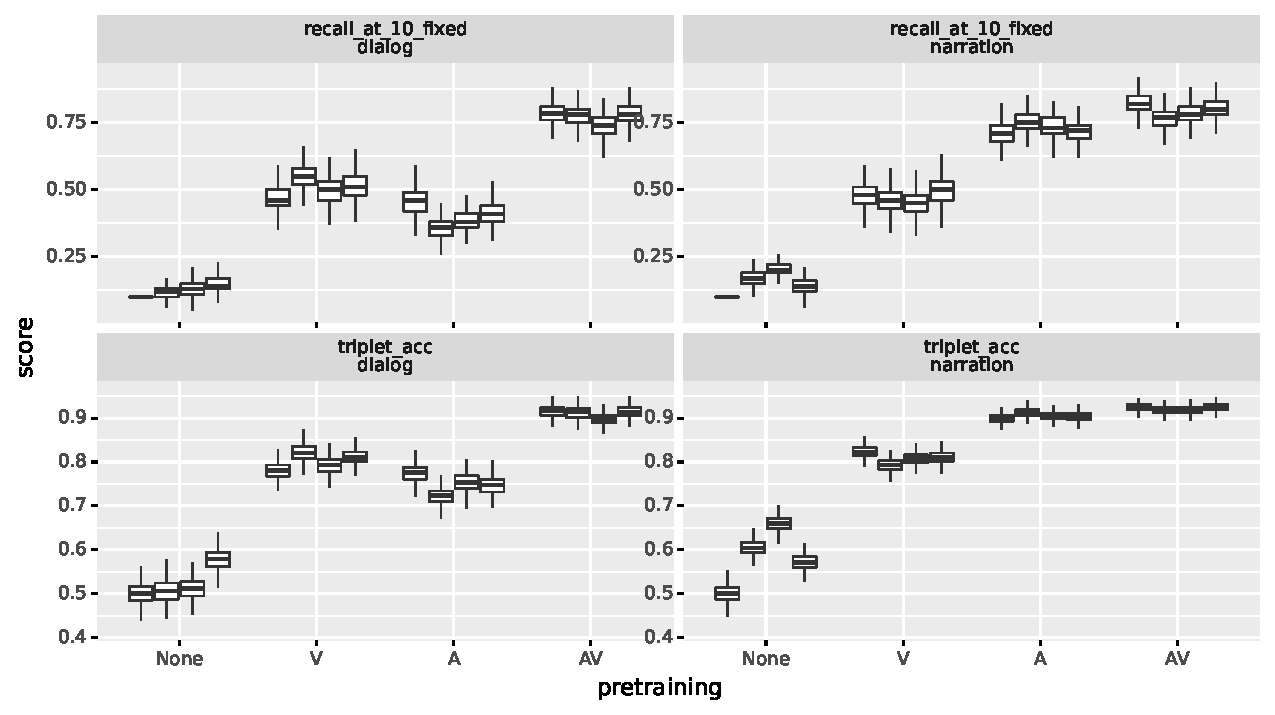
\includegraphics[width=\columnwidth]{results/ablations/pretraining.pdf}
	\caption{Effect of pre-training.}
	\label{fig:pretraining}
\end{figure}

\begin{figure}[htb]
  \centering
  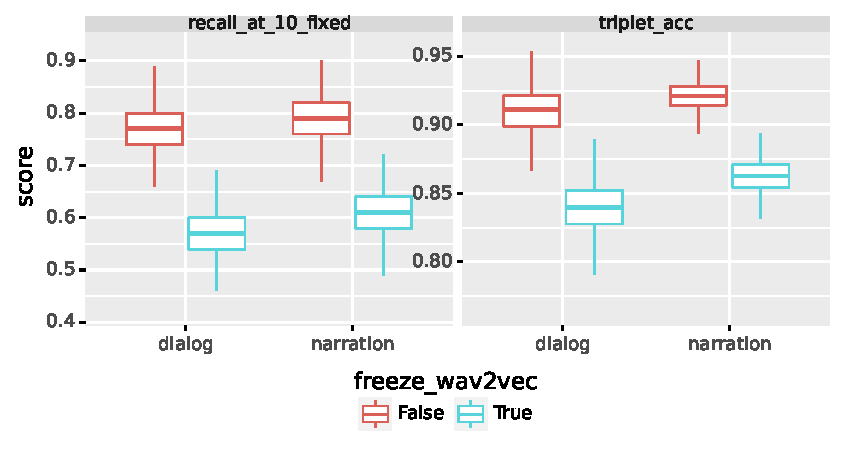
\includegraphics[width=\columnwidth]{results/ablations/freeze_wav2vec.pdf}
  \caption{Effect of freezing the parameters of the \textsc{wav2vec} module.}
  \label{fig:freeze_wav2vec}
\end{figure}


\begin{figure}[htb]
	\centering
	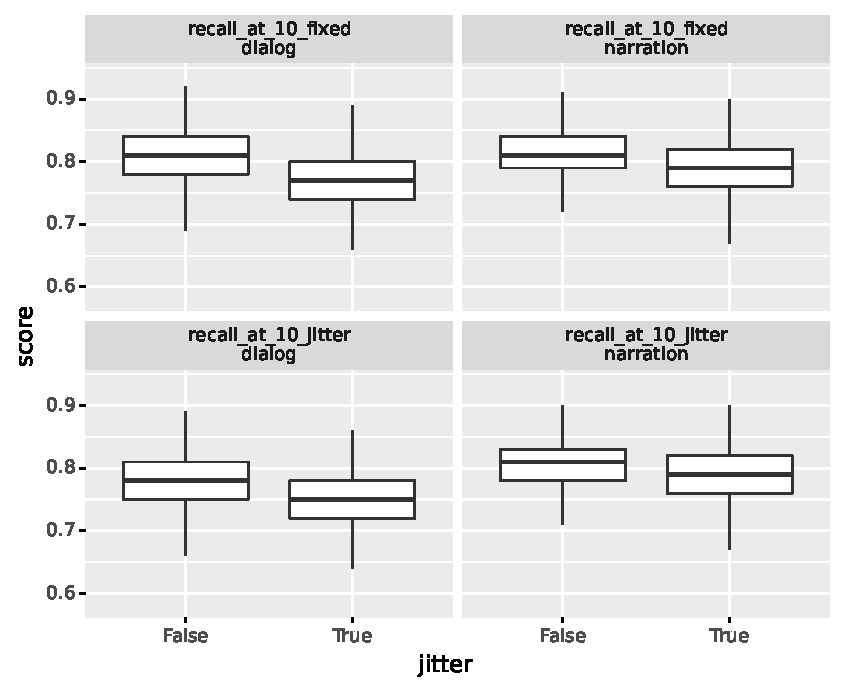
\includegraphics[width=\columnwidth]{results/ablations/jitter.pdf}
	\caption{Effect of jitter.}
	\label{fig:jitter}
\end{figure}

\begin{figure}[htb]
  \centering
  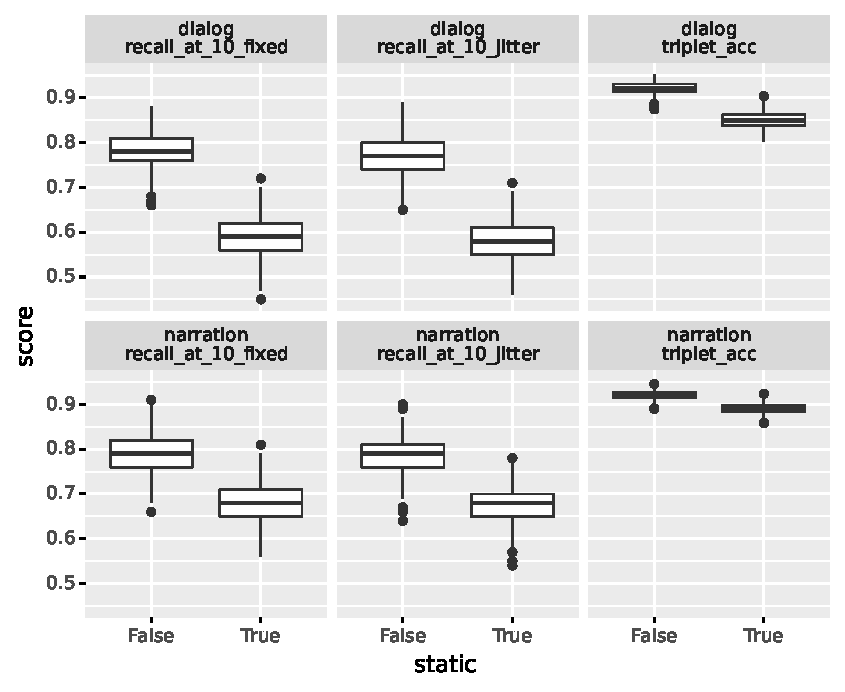
\includegraphics[width=\columnwidth]{results/ablations/static.pdf}
  \caption{Effect of temporal information.}
  \label{fig:static}
\end{figure}


\subsection{Minimal Pairs}
As a first baseline, we evaluate a model that has been pretrained but not fine-tuned on our dataset. The resulting performance is, as expected, close to chance level: 0.538.\todo{MN: add baselines: model that is completely untrained, and model where only the attention pooling layers are finetuned} Additionally, we evaluate a model that is trained using static (image) data instead of video. The average accuracy is 0.705 . Finally, the best performing model according to the
performance metrics (ID 68, audio and video pretraining) achieves an average
targeted triplets accuracy of 0.745.

\Cref{fig:accuracy_targeted_triplets_nouns} and
\ref{fig:accuracy_targeted_triplets_verbs} show per-word
accuracy for nouns and verbs, respectively. We perform boostrapping (n\_resampling = 100) to estimate mean and standard deviation for each accuracy score.

We further compute correlations between the per-word accuracy and two 
possible predictors of age of acquisition: frequency and concreteness. 
We do not find any significant correlation between the model's per-word 
accuracy and word concreteness or input frequency of a word in the 
training data.\todo{MN: verify correlations for final versions}




\begin{figure*}[htb]
  \centering
  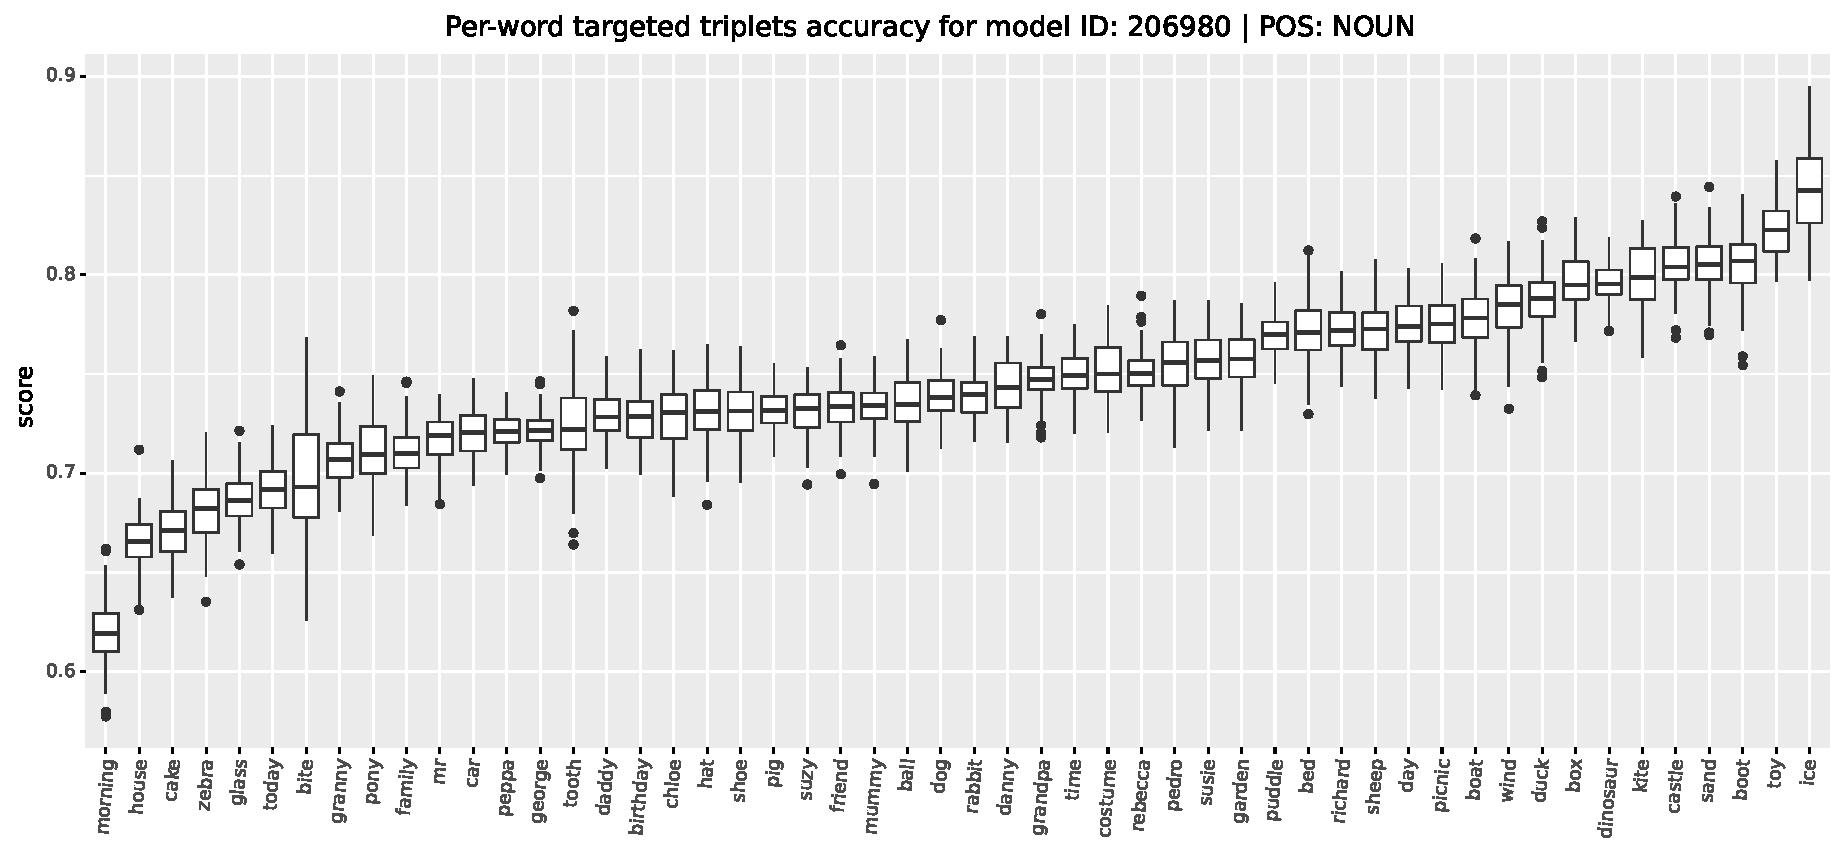
\includegraphics[width=\textwidth]{results/targeted_triplets/results_per_word_version_206980_NOUN.pdf}
  \caption{Per-word targeted triplets accuracy for nouns.}
  \label{fig:accuracy_targeted_triplets_nouns}
\end{figure*}

\begin{figure*}[htb]
  \centering
  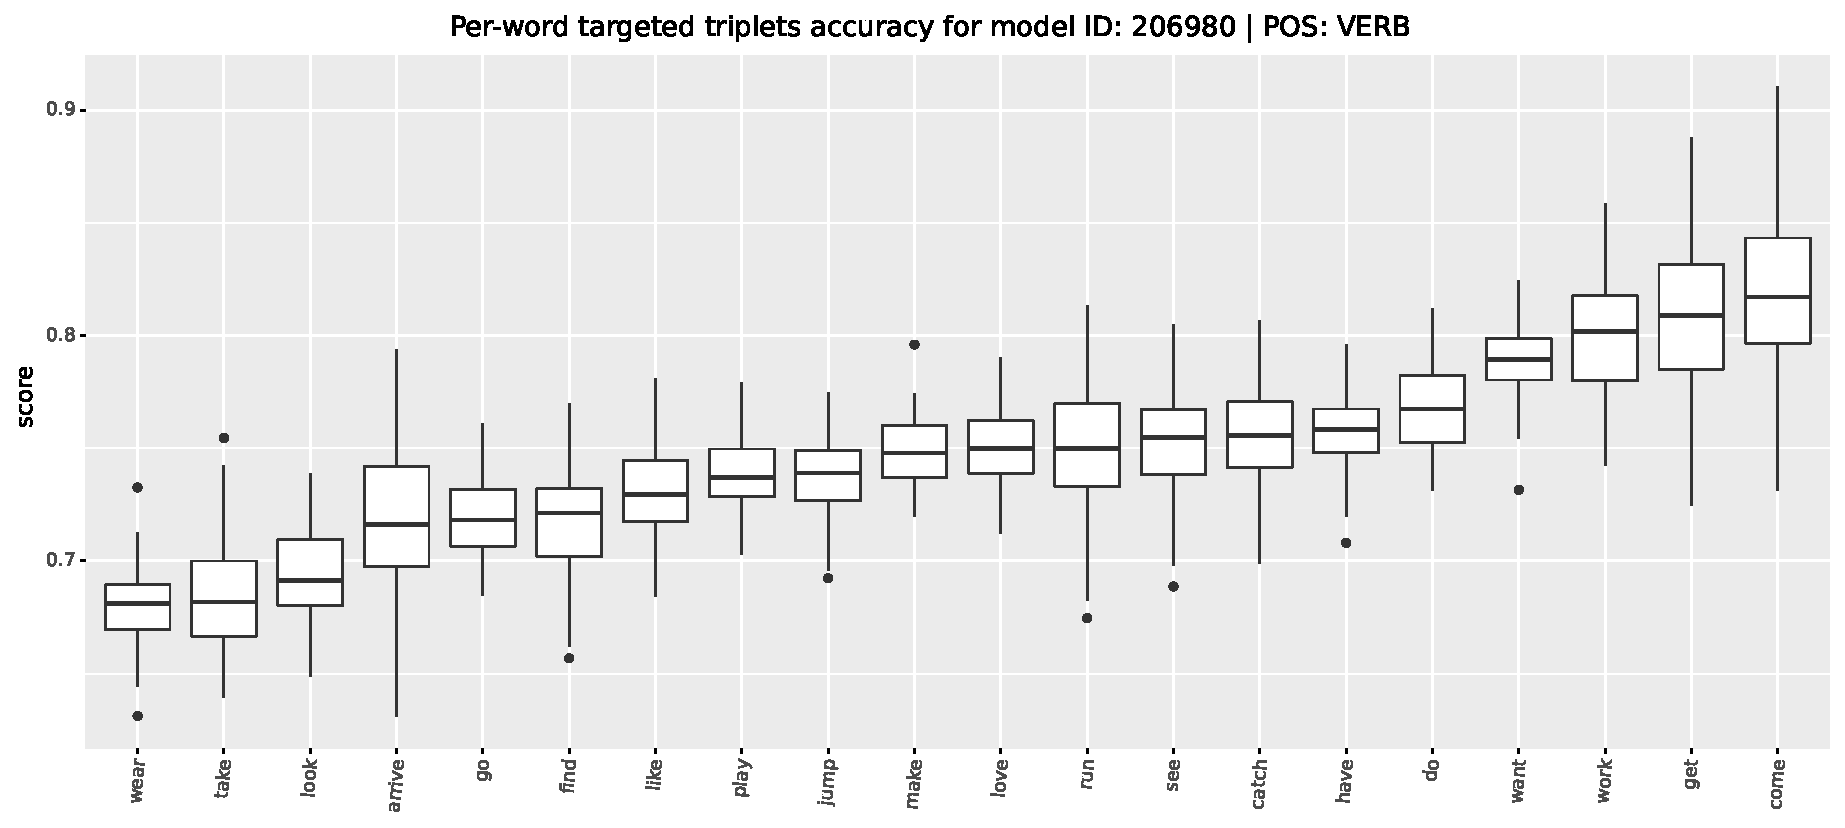
\includegraphics[width=\textwidth]{results/targeted_triplets/results_per_word_version_206980_VERB.pdf}
  \caption{Per-word targeted triplets accuracy for verbs.}
  \label{fig:accuracy_targeted_triplets_verbs}
\end{figure*}
